%!TEX root = ../../Heun_Dale_Haney_A_dynamic_approach_to_input_output_modeling.tex
%%%%%%%%%%%%%%%%%%%%% chapter.tex %%%%%%%%%%%%%%%%%%%%%%%%%%%%%%%%%
%
% sample chapter
%
% Use this file as a template for your own input.
%
%%%%%%%%%%%%%%%%%%%%%%%% Springer-Verlag %%%%%%%%%%%%%%%%%%%%%%%%%%
%\motto{Use the template \emph{chapter.tex} to style the various elements of your chapter content.}

%%%%%%%%%%%%%%%%%%%%%%%%%%%%%%%%%%%%%%
%%%%%%%%%% Energy Intensity %%%%%%%%%%
%%%%%%%%%%%%%%%%%%%%%%%%%%%%%%%%%%%%%%
\chapter{Energy intensity}
% Always give a unique label
\label{chap:intensity} 
% use \chaptermark{} to alter or adjust the chapter heading in the running head
\chaptermark{intensity}
%%%%%%%%%%%%%%%%%%%%%%%%%%%%%%%%%%
%%%%%%%%%%%%%%%%%%%%%%%%%%%%%%%%%%
%%%%%%%%%%%%%%%%%%%%%%%%%%%%%%%%%%

\abstract*{[NEED TO ADD ABSTRACT HERE]}

%% \abstract{Each chapter should be preceded by an abstract (10--15 lines long) that summarizes the content. The abstract will appear \textit{online} at \url{www.SpringerLink.com} and be available with unrestricted access. This allows unregistered users to read the abstract as a teaser for the complete chapter. As a general rule the abstracts will not appear in the printed version of your book unless it is the style of your particular book or that of the series to which your book belongs.\newline\indent
%% Please use the 'starred' version of the new Springer \texttt{abstract} command for typesetting the text of the online abstracts (cf. source file of this chapter template \texttt{abstract}) and include them with the source files of your manuscript. Use the plain \texttt{abstract} command if the abstract is also to appear in the printed version of the book.}

%% Use the template \emph{chapter.tex} together with the Springer document class SVMono (monograph-type books) or SVMult (edited books) to style the various elements of your chapter content in the Springer layout.


In Chapters~\ref{chap:direct_energy},~\ref{chap:embodied_energy}, and~\ref{chap:value}, 
we defined flows of direct energy, embodied energy, and value in an economy.
In this chapter, we merge energy and value together to estimate
the energy intensity ($\varepsilon$) of economic sectors.\footnote{The literature discusses 
the energy embodied in \emph{products}, e.g.\ ``The data and methodologies described in this report 
permit calculation of five types of energy `embodied' 
in a particular goods~[\emph{sic}] or service,'' % chktex 38
from Bullard~\cite[p.~268]{Bullard:1978vd}. 
It can be meaningful to discuss the energy intensity of \emph{processes}, too,
and we switch between these two meanings of the word ``embodied.''}


%%%%%%%%%% Methodology %%%%%%%%%%
\section{Methodology}
%%%%%%%%%%

Energy intensity ($\varepsilon$)\nomenclature[e]{$\varepsilon$}{energy intensity [J/\$]}
\index{energy intensity}
is the ratio 
of total energy ($\dot{T}$) 
and value ($\dot{X}$) outflow rates 
from an economic sector, 
such that for the $j^{\mathrm{th}}$ goods and services sector,

\begin{equation} \label{eq:epsilon_output_def_g_and_s}
	\varepsilon_{j} \equiv \frac{\dot{T}_{j}}{\dot{X}_{j}},
\end{equation} 

\noindent{}and $\varepsilon$ is in units of J/\$.\footnote{It may be
instructive to consider energy intensity as the quotient
of embodied energy (in units of J/kg) and price (in \$/kg).}
Equation~\ref{eq:epsilon_output_def_g_and_s}
includes the embodied energy of products in the numerator ($\dot{T}_{j}$) term. 
A narrower definition ef energy intensity would be 
$\varepsilon_{j}~\equiv~\frac{\dot{Q}_{j0}}{\dot{X}_{j}}$,
which includes only direct energy consumed by the sector
in the numerator
and excludes the energy demanded upstream by the 
resource flows ($\dot{R}$) that comprise the product of the sector ($\dot{P}$).
We choose the broader definition of
Equation~\ref{eq:epsilon_output_def_g_and_s},
because it accounts for upstream energy consumption,
thereby providing an estimate of the true energy cost of products.
For inter-sector flows, we have

\begin{equation} \label{eq:epsilon_transfers_1}
	\varepsilon_{jk} = \frac{\dot{T}_{jk}}{\dot{X}_{jk}}.
\end{equation}

\noindent{}Furthermore, we note that 

\begin{equation} \label{eq:epsilon_equiv_1}
	\varepsilon_{j} = \varepsilon_{jk}
\end{equation}

\noindent{}for all $k$, because the energy intensity 
of sector $j$'s output is independent of its destination ($k$). 
All goods produced by a sector 
are produced at the average energy intensity 
of that sector.\footnote{If this approach is unsatisfactory, 
the sector may be divided into sub-sectors 
with different energy intensities.}

We define the input-ouput ratio ($a_{ij}$)\nomenclature[a]{$a$}{input-output ratio [-]}
that represents the input 
of good $i$ required to produce a unit of output from sector $j$.

\begin{equation} \label{eq:aij_def}
	a_{ij} \equiv \frac{\dot{X}_{ij}}{\dot{X}_{j}}
\end{equation}

Input-output ratios are given in mixed units, 
depending on both the purpose of each sector of the economy 
and the type of input as shown in Figure~\ref{fig:A_matrix_units}.

\begin{figure}[h!]
\centering\
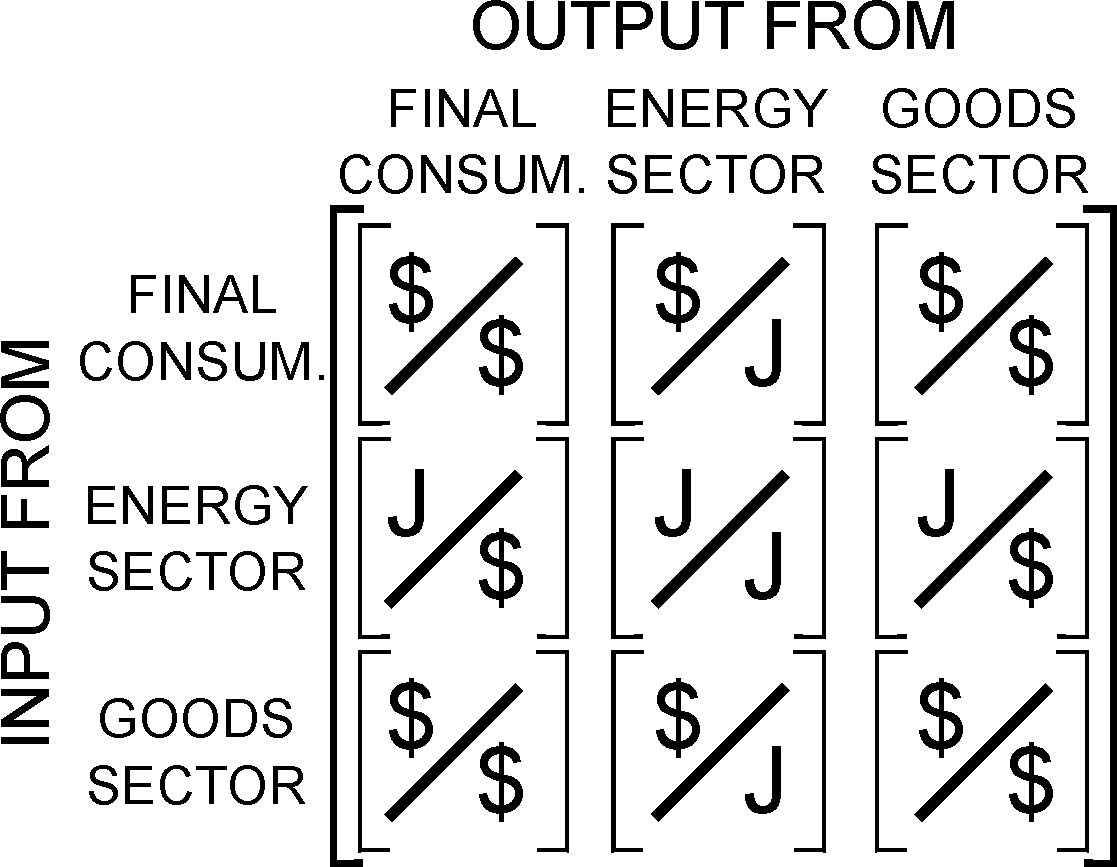
\includegraphics[width=0.4\linewidth]{Part_2/Chapter_Intensity/images/I-O_units.pdf}
\caption[Units for input-output ratios]{ Units for input-output ratios ($a$).}
\label{fig:A_matrix_units}
\end{figure}

Equations~\ref{eq:epsilon_transfers_1}, 
\ref{eq:epsilon_equiv_1}, and 
\ref{eq:aij_def} can be combined to give

\begin{equation}
	\dot{T}_{jk} = \varepsilon_{j} a_{jk} \dot{X}_{k}.
\end{equation}


%%%%%%%%%% Example A %%%%%%%%%%
\section{Example A: single-sector economy} % chktex 13
%%%%%%%%%%

With reference to Figures~\ref{fig:A_energy}, 
\ref{fig:A_total_energy_T_dot}, 
and~\ref{fig:A_value},
the energy intensity ($\varepsilon_{1}$) of a single-sector economy is calculated by

\begin{equation} \label{eq:A-energy_intensity}
	\varepsilon_{1} 
	= \frac{\dot{T}_{1}}{\dot{X}_{1}} 
	= \frac{\dot{T}_{11}}{\dot{X}_{11}}.
\end{equation}

Appendix~\ref{chap:infinite_series} illustrates that the energy 
intensity of a single-sector economy ($\varepsilon_{1}$) 
is comprised of the sum of the infinite recursions
of energy consumed during production of output ($\dot{X}_{1}$).

To estimate energy intensities
when more than one economic sector is involved, 
we move to Examples~B and~C in the following sections.


%%%%%%%%%% Example B %%%%%%%%%%
\section{Example B: two-sector economy} % chktex 13
%%%%%%%%%%

With reference to Figures~\ref{fig:B_energy}, 
\ref{fig:B_total_energy},
and~\ref{fig:B_value}, 
the energy intensity ($\varepsilon_{2}$) 
of the production sector is given by

\begin{equation} \label{eq:single_sector_energy_intensity}
	\varepsilon_{2} 
	= \frac{\dot{T}_{2}}{\dot{X}_{2}} 
	= \frac{\dot{T}_{22}}{\dot{X}_{22}}.
\end{equation}

\noindent{}Thus,

\begin{equation} \label{eq:T_dot_1_single_sector}
	\dot{T}_{2} = \varepsilon_{2}\dot{X}_{2},
\end{equation}

The input-output ratio 
for the production sector's self-use of output ($a_{22}$) is

\begin{equation} \label{eq:io_ratio_single_sector}
	a_{22} = \frac{\dot{X}_{22}}{\dot{X}_{2}},
\end{equation}

\noindent{}thus

\begin{equation} \label{eq:T_dot_11_single_sector}
	\dot{T}_{22} = \varepsilon_{2}a_{22}\dot{X}_{2}.
\end{equation}

We can rewrite the total energy accounting equation 
for the two-sector economy

\begin{equation}
	\frac{\mathrm{d}T_{2}}{\mathrm{d}t} 	 
	= \dot{T}_{02} 
	+ \dot{T}_{12}
	+ \dot{T}_{22} 
	- \dot{T}_{2} 
	- \dot{T}_{20} \tag{\ref{eq:CV_T_2}}
\end{equation}

\noindent{}using energy intensity by realizing that 

\begin{itemize}
	\item{$\frac{\mathrm{d}E_2}{\mathrm{d}t} = 0$
		and
		$\frac{\mathrm{d}T_2}{\mathrm{d}t} = \frac{\mathrm{d}B_2}{\mathrm{d}t}$, 
		because direct energy
		does not accumulate within economic sectors,}
	\item{$\frac{\mathrm{d}B_2}{\mathrm{d}t} = \frac{\mathrm{d}B_{K_{2}}}{\mathrm{d}t}$,
		because resources ($R$) and short-lived materials ($S$) do not 
		accumulate at appreciable rates in economic sectors,}
	\item{$\dot{B}_{02} = 0$ and $\dot{T}_{02} = \dot{E}_{02}$,
		because embodied energy appears only in the \emph{output} of a sector,}
	\item{$\dot{E}_{20} = 0$ and $\dot{T}_{20} = \dot{B}_{20}$, 
	because direct energy is not wasted to the biosphere at any significant rate, and} 
	\item{$\dot{B}_{20} = \left( \dot{B}_{\dot{R}_{20}} 
							+ \dot{B}_{\dot{S}_{20}}
							+ \dot{B}_{\dot{K}_{20}}
							\right)
						= \left( \dot{B}_{\dot{R}_{20}} 
							+ \dot{B}_{\dot{S}_{20}}
							+ \gamma_{K,2} B_{K_{2}}
							\right)$, as shown in Section~\ref{sec:Embodied_Energy_Example_C}.}
\end{itemize}

\noindent{}If we substitute Equations~\ref{eq:T_dot_1_single_sector} 
and~\ref{eq:T_dot_11_single_sector} into Equation~\ref{eq:CV_T_2}, we obtain

\begin{equation} \label{eq:dB1/dt_single_sector_after_substituting_eps_and_a}
	\frac{\mathrm{d}B_{K_{2}}}{\mathrm{d}t} 
	= \dot{E}_{02} 
	+ \dot{T}_{12}
	+ \varepsilon_{2}a_{22}\dot{X}_{2} 
	- \varepsilon_{2}\dot{X}_{2} 
	- \left( \dot{B}_{\dot{R}_{20}} 
							+ \dot{B}_{\dot{S}_{20}}
							+ \gamma_{K,2} B_{K_{2}}
							\right).
\end{equation}

Equation~\ref{eq:dB1/dt_single_sector_after_substituting_eps_and_a}
can be solved for energy intensity ($\varepsilon_{2}$) to obtain

\begin{equation} \label{eq:B-epsilon}
	\varepsilon_{2}
	= {(1 - a_{22})}^{-1} {\dot{X}_{2}}^{-1} 
		\left[
			\dot{E}_{02}
			+ \dot{T}_{12}
			- \frac{\mathrm{d}B_{K_{2}}}{\mathrm{d}t} 
			- \dot{B}_{\dot{R}_{20}}
			- \dot{B}_{\dot{S}_{20}}
			- \gamma_{K,2} B_{K_{2}}
		\right]
\end{equation}

To extend Equation~\ref{eq:B-epsilon}
to a matrix formulation, we turn to Example~C.


%%%%%%%%%% Example C %%%%%%%%%%
\section{Example~C: three-sector economy} % chktex 13
\label{sec:C-intensity}
%%%%%%%%%%

The three-sector economy of Example~C affords the opportunity 
to develop a matrix version 
of the total energy accounting equation (\ref{eq:C-CV_T_123})
and to develop an equation that estimates the
energy intensity of economic sectors. 
We begin with a matrix version of the total energy accounting equation.


%+++++++++ Example C: Total energy equation ++++++++++
\subsection{Total energy accounting equation}
%+++++++++

We apply Equation~\ref{eq:C-CV_T_123} to the three-sector
economy shown in 
Figures~\ref{fig:C_energy},~\ref{fig:C_total_energy}, and~\ref{fig:C_value}
to obtain the following total energy accounting equations
for the Energy~(2) and Goods and Services~(3) sectors 
of the three-sector economy:

\begin{equation} \label{eq:C-Total_Energy_Sec_2-a}
	\frac{\mathrm{d}T_{2}}{\mathrm{d}t} 
	= \dot{T}_{02}  
	+ \dot{T}_{12}
	+ \dot{T}_{22}
	+ \dot{T}_{32}
	- \dot{T}_{2}
	- \dot{T}_{20}
\end{equation}

\noindent{}and

\begin{equation} \label{eq:C-Total_Energy_Sec_3-a}
	\frac{\mathrm{d}T_{3}}{\mathrm{d}t} 
	= \dot{T}_{03}  
	+ \dot{T}_{13}
	+ \dot{T}_{23}
	+ \dot{T}_{33}
	- \dot{T}_{3}
	- \dot{T}_{30}.
\end{equation}

\noindent{}Similar to Example~B, we realize that 

\begin{itemize}
	\item{$\frac{\mathrm{d}E_i}{\mathrm{d}t} = 0$
		and
		$\frac{\mathrm{d}T_i}{\mathrm{d}t} = \frac{\mathrm{d}B_i}{\mathrm{d}t}$, 
		because direct energy
		does not accumulate within economic sectors,}
	\item{$\frac{\mathrm{d}B_i}{\mathrm{d}t} = \frac{\mathrm{d}B_{K_{i}}}{\mathrm{d}t}$,
		because resources ($R$) and short-lived materials ($S$) do not 
		accumulate at appreciable rates in economic sectors,}
	\item{$\dot{B}_{0j} = 0$ and $\dot{T}_{0j} = \dot{E}_{0j}$,
		because embodied energy appears only in the \emph{output} of a sector,}
	\item{$\dot{E}_{j0} = 0$ and $\dot{T}_{j0} = \dot{B}_{j0}$, 
	because direct energy is not wasted to the biosphere at any significant rate, and} 
	\item{$\dot{B}_{j0} = \left( \dot{B}_{\dot{R}_{j0}} 
							+ \dot{B}_{\dot{S}_{j0}}
							+ \dot{B}_{\dot{K}_{j0}}
							\right)
						= \left( \dot{B}_{\dot{R}_{j0}} 
							+ \dot{B}_{\dot{S}_{j0}}
							+ \gamma_{K,j} B_{K_{j}}
							\right)$, as shown in Section~\ref{sec:Embodied_Energy_Example_C}.}
\end{itemize}

\noindent{}to obtain

\begin{equation} \label{eq:C-Total_Energy_Sec_2-b}
	\frac{\mathrm{d}B_{K_{2}}}{\mathrm{d}t}
	= \dot{E}_{02}
	+ \dot{T}_{12}
	+ \varepsilon_{2} \dot{X}_{22}
	+ \varepsilon_{3} \dot{X}_{32}
	- \varepsilon_{2} \dot{X}_{2}
	- \left( \dot{B}_{\dot{R}_{20}} 
							+ \dot{B}_{\dot{S}_{20}}
							+ \gamma_{K,2} B_{K_{2}}
							\right)
\end{equation}

\noindent{}and

\begin{equation} \label{eq:C-Total_Energy_Sec_3-b}
	\frac{\mathrm{d}B_{K_{3}}}{\mathrm{d}t}
	= \dot{E}_{03}
	+ \dot{T}_{13}
	+ \varepsilon_{2} \dot{X}_{23}
	+ \varepsilon_{3} \dot{X}_{33}
	- \varepsilon_{3} \dot{X}_{3}
	- \left( \dot{B}_{\dot{R}_{30}} 
							+ \dot{B}_{\dot{S}_{30}}
							+ \gamma_{K,3} B_{K_{3}}
							\right).
\end{equation}


%%%%%%%%%% Example C: Matrix formulation %%%%%%%%%%
\subsection{Matrix formulation} % chktex 13
\label{sec:C-matrix}
%%%%%%%%%%

Equations~\ref{eq:C-Total_Energy_Sec_2-b} 
and~\ref{eq:C-Total_Energy_Sec_3-b} can be rewritten 
in vector notation as

\begin{equation} \label{eq:C-Expanded_Matrix_Form}
	\begin{split}
		\begin{Bmatrix}
			\frac{\mathrm{d}B_{K_{2}}}{\mathrm{d}t} \\[0.4em] % Adds some vertical space.
			\frac{\mathrm{d}B_{K_{3}}}{\mathrm{d}t} 
		\end{Bmatrix}
		=
		\begin{Bmatrix}
			\dot{E}_{02}\\
			\dot{E}_{03}
		\end{Bmatrix}
		& +                                               % & sets alighment tab
		\begin{Bmatrix}
			\dot{T}_{12}\\
			\dot{T}_{13}
		\end{Bmatrix}
		+
		\begin{bmatrix}
			\dot{X}_{22} & \dot{X}_{32}\\
			\dot{X}_{23} & \dot{X}_{33}
		\end{bmatrix}
		\begin{Bmatrix}
			\varepsilon_{2}\\
			\varepsilon_{3}
		\end{Bmatrix}   
		- 
		\begin{bmatrix}
			\dot{X}_{2} & 0          \\
			0           & \dot{X}_{3}
		\end{bmatrix}
		\begin{Bmatrix}
			\varepsilon_{2}\\
			\varepsilon_{3}
		\end{Bmatrix} \\                                 % \\ gives line break
		& -                                              % & aligns to previous tab
		\begin{Bmatrix}
			\dot{B}_{\dot{R}_{20}}  \\
			\dot{B}_{\dot{R}_{30}} 
		\end{Bmatrix}
		-
		\begin{Bmatrix}
			\dot{B}_{\dot{S}_{20}}  \\
			\dot{B}_{\dot{S}_{30}} 
		\end{Bmatrix}
		-
		\begin{bmatrix}
			\gamma_{K,2} & 0          \\
			0            & \gamma_{K,3}
		\end{bmatrix}
		\begin{Bmatrix}
			B_{K_{2}}\\
			B_{K_{3}}
		\end{Bmatrix}.
	\end{split}
\end{equation}

\noindent{}If we define the following matrices and vectors:

\begin{equation} \label{eq:B_vec_def}
	\vec{B}_{K} 
	\equiv
	\begin{Bmatrix}	
		B_{K_{2}} \\
		B_{K_{3}}
	\end{Bmatrix},
\end{equation}

\begin{equation} \label{eq:dBdt_vec_def}
	\frac{\mathrm{d}\vec{B}_K}{\mathrm{d}t} 
	\equiv
	\begin{Bmatrix}	
		\frac{\mathrm{d}B_{K_{2}}}{\mathrm{d}t}	\\[0.4em] % Adds some vertical space.
		\frac{\mathrm{d}B_{K_{3}}}{\mathrm{d}t}
	\end{Bmatrix},
\end{equation}

\begin{equation} \label{eq:E_vec_def}
	\vec{E}_{0} 
	\equiv
	\begin{Bmatrix}
		\dot{E}_{02} \\
		\dot{E}_{03}
	\end{Bmatrix},
\end{equation} \nomenclature[E]{$\vec{E}_{0}$}{vector of direct energy inputs 
												from the biosphere [W]}

\begin{equation} \label{eq:T_vec_def}
	\vec{T}_{1} 
	\equiv
	\begin{Bmatrix}
		\dot{T}_{12} \\
		\dot{T}_{13}
	\end{Bmatrix},
\end{equation} \nomenclature[T]{$\vec{T}_{1}$}{vector of total energy inputs 
												from society to the economy [W]}

\begin{equation} \label{eq:X_t_matrix_def}
	\vec{X}_{t} 
	\equiv
	\begin{bmatrix}
		\dot{X}_{22} & \dot{X}_{23} \\
		\dot{X}_{32} & \dot{X}_{33}
	\end{bmatrix},
\end{equation} \nomenclature[X]{$\vec{X}_{t}$}{transaction matrix [\$/year]}
\index{transaction matrix}\index{matrix!transaction|see{transaction matrix}}

\begin{equation} \label{eq:eps_vec_def}
	\bm{\varepsilon} 
	\equiv
	\begin{Bmatrix}
		\varepsilon_{2}	\\
		\varepsilon_{3}
	\end{Bmatrix},
\end{equation} \nomenclature[e]{$\bm{\varepsilon}$}{column vector 
								of sector energy intensities [J/\$]}
								
\begin{equation} \label{eq:waste_vec_def}
	\vec{B}_{waste} 
	=
	\begin{Bmatrix}
		\dot{B}_{waste,{20}}	\\
		\dot{B}_{waste,{30}}	\\
	\end{Bmatrix}
	\equiv
	\begin{Bmatrix}
		\dot{B}_{\dot{R}_{20}}	\\
		\dot{B}_{\dot{R}_{30}}	\\
	\end{Bmatrix}
	+
	\begin{Bmatrix}
		\dot{B}_{\dot{S}_{20}}	\\
		\dot{B}_{\dot{B}_{30}}	\\
	\end{Bmatrix},
\end{equation} \nomenclature[B]{$\vec{B}_{waste}$}{column vector 
								of waste embodied energy from resource ($\dot{R}$)
								and short-lived material ($\dot{S}$) flow [J/s]}

\begin{equation} \label{eq:X_hat_matrix_def}
	\hat{\vec{X}} 
	\equiv
	\delta_{ij} \dot{X}_{j} 
	= 
	\begin{bmatrix}
		\dot{X}_{2}		&	0	  \\
		0				&	\dot{X}_{3}	\\
	\end{bmatrix},
\end{equation} \nomenclature[X]{$\hat{\vec{X}}$}{matrix of sector outputs [\$/year]}

\noindent{}and

\begin{equation} \label{eq:gamma_hat_matrix_def}
	\hat{\bm{\gamma}}_{K}
	\equiv
	\delta_{ij} \gamma_{K,j}
	=
	\begin{bmatrix}
		\gamma_{K,2} & 0         \\
		0            & \gamma_{K,3}
	\end{bmatrix};
\end{equation}\nomenclature[g]{$\hat{\bm{\gamma}}$}{matrix of depreciation rates [\$/year]}

\noindent{}with the ``Kronecker delta''

\begin{equation}\label{eq:k_delta}
	\delta_{ij} 
	\equiv
	\begin{cases}	
		0	&	\text{if  } i \neq j	\\
		1 	& 	\text{if  } i = j
	\end{cases};
\end{equation}\nomenclature[d]{$\delta_{ij}$}{Kronecker delta}

\noindent{}we can rewrite Equation~\ref{eq:C-Expanded_Matrix_Form}
compactly as

\begin{equation} \label{eq:matrix_leontief_pre_1}
	\frac{\mathrm{d}\vec{B}_{K}}{\mathrm{d}t} 
	= \vec{E}_{0}
	+ \vec{T}_{1}
	+ \vec{X}_{t}^{\mathrm{T}}\bm{\varepsilon} 
	- \hat{\vec{X}}\bm{\varepsilon}
	- \vec{B}_{waste}
	- \hat{\bm{\gamma}}_{K} \vec{B}_{K}.
\end{equation}

\noindent{}Equation~\ref{eq:matrix_leontief_pre_1} can be simplified to

\begin{equation} \label{eq:matrix_leontief_pre_2}
	\frac{\mathrm{d}\vec{B}_{K}}{\mathrm{d}t} 
	= \vec{E}_{0}
	+ \vec{T}_{1}
	+ (\vec{X}_{t}^{\mathrm{T}} - \hat{\vec{X}})\bm{\varepsilon} 
	- \vec{B}_{waste}
	- \hat{\bm{\gamma}}_{K}\vec{B}_{K}.
\end{equation}

\noindent{}We can define the input-output matrix ($\vec{A}$) as

\begin{equation} \label{eq:A_matrix_def}
	\vec{A} 
	\equiv
	\begin{bmatrix}
		a_{22} & a_{23}	\\
		a_{32} & a_{33}	
	\end{bmatrix}.
\end{equation} \nomenclature[A]{$\vec{A}$}{input-output matrix [-]}
\index{input-output matrix}\index{matrix!input-output|see{input-output matrix}}

\noindent{}Appendix~\ref{app:Proof} shows that

\begin{equation} \label{eq:Xdifference1}
	\vec{X}_{t}^{\mathrm{T}} 
	- \hat{\vec{X}} 
	= \hat{\vec{X}} (\vec{A}^{\mathrm{T}} - \vec{I}),
\end{equation}

\noindent{}which allows Equation~\ref{eq:matrix_leontief_pre_2}
to be recast as

\begin{equation} \label{eq:matrix_leontief}
	\frac{\mathrm{d}\vec{B}_{K}}{\mathrm{d}t} 
	= \vec{E}_{0}
	+ \vec{T}_{1}
	+ \hat{\vec{X}} (\vec{A}^{\mathrm{T}} - \vec{I})\bm{\varepsilon} 
	- \vec{B}_{waste}
	- \hat{\bm{\gamma}}_{K}\vec{B}_{K}.
\end{equation}

\noindent{}Equation~\ref{eq:matrix_leontief} is the matrix version 
of the total energy accounting equation
written in terms of embodied energy ($\vec{B}$), 
energy intensities ($\bm{\varepsilon}$),
and input-output ratios ($\vec{A}$).
Equation~\ref{eq:C-Expanded_Matrix_Form} applies 
for the three-sector economy of Example~C, 
but the equivalent matrix formulation (Equation~\ref{eq:matrix_leontief}) 
can be extended to any desired level 
of economic and energy sector disaggregation 
by expanding the vectors and matrices in 
Equations~\ref{eq:dBdt_vec_def}--\ref{eq:B_vec_def}
and~\ref{eq:A_matrix_def} to include
all sectors of the economy.\cite{Bullard:1978vd,Casler1984}

Equation~\ref{eq:matrix_leontief} provides a means to 
estimate the embodied energy accumulation rate
in economic sectors $\left(\frac{\mathrm{d}\vec{B}_{K}}{\mathrm{d}t}\right)$ 
knowing only 
direct energy inputs to the economy from the biosphere ($\vec{E}_{0}$), 
total energy inputs from society to the economy ($\vec{T}_{1}$),
sector outputs ($\hat{\vec{X}}$), 
sector input-output ratios ($\vec{A}$), 
sector energy intensities ($\bm{\varepsilon}$), 
energy embodied in wastes from the economy ($\vec{B}_{waste}$),
and physical depreciation rates of capital stock ($\hat{\bm{\gamma}}_{K}\vec{B}_{K}$). 
In theory, the transaction matrix ($\vec{X}_{t}$) is not required 
if the input-ouput matrix ($\vec{A}$) is known, 
though in practice, 
knowledge of input-output matrix ($\vec{A}$) 
would be derived from the transaction matrix ($\vec{X}_{t}$),
as shown in Appendix~\ref{chap:Estimating_A}.


% %%%%%%%%%% Example C %%%%%%%%%%
% \section{Estimating $\bm{\varepsilon}$}
% \label{sec:estimating_epsilon-intensity_chapter}
% %%%%%%%%%%

Equation~\ref{eq:matrix_leontief} can be rearranged to obtain

\begin{equation} \label{eq:epsilon_derivation_1}
	\hat{\vec{X}} (\vec{A}^{\mathrm{T}} - \vec{I}) \bm{\epsilon}
	= \frac{\mathrm{d}\vec{B}_{K}}{\mathrm{d}t}
	+ \vec{B}_{waste}
	+ \hat{\bm{\gamma}}_{K} \vec{B}_{K}
	- \vec{E}_{0}
	- \vec{T}_{1} 
\end{equation}

\noindent{}and

\begin{equation} \label{eq:epsilon_derivation_2}
	\bm{\epsilon}
	= {\left[ \hat{\vec{X}} (\vec{A}^{\mathrm{T}} - \vec{I}) \right]}^{-1}
		\left[
			\frac{\mathrm{d}\vec{B}_{K}}{\mathrm{d}t}
			+ \vec{B}_{waste}
			+ \hat{\bm{\gamma}}_{K} \vec{B}_{K}
			- \vec{E}_{0}
			- \vec{T}_{1} 
		\right].
\end{equation}

\noindent{}We apply the matrix identity 
from Formula 6.2, p. 308 in Beyer~\cite{Beyer:1991vd}

\begin{equation} \label{eq:matrix_identity_Beyer}
	{\left(\vec{A}\vec{B}\vec{C}\right)}^{-1} 
	= \vec{C}^{-1} \vec{B}^{-1} \vec{A}^{-1}
\end{equation}

\noindent{}to the right side of Equation~\ref{eq:epsilon_derivation_2} to obtain

\begin{equation} \label{eq:epsilon_derivation_3}
	\bm{\epsilon}
	= {(\vec{A}^{\mathrm{T}} - \vec{I})}^{-1} {\hat{\vec{X}}}^{-1} 
		\left[
			\frac{\mathrm{d}\vec{B}_{K}}{\mathrm{d}t}
			+ \vec{B}_{waste}
			+ \hat{\bm{\gamma}}_{K} \vec{B}_{K}
			- \vec{E}_{0}
			- \vec{T}_{1} 
		\right].
\end{equation}

\noindent{}Finally, we can multiply both parenthetical terms\footnote{The parenthetical
terms on the right side of Equation~\ref{eq:epsilon_derivation_3} 
are $(\vec{A}^{\mathrm{T}} - \vec{I})$ and
$
\left[
	\frac{\mathrm{d}\vec{B}_{K}}{\mathrm{d}t}
	+ \vec{B}_{waste}
	+ \hat{\bm{\gamma}}_{K} \vec{B}_{K}
	- \vec{E}_{0}
	- \vec{T}_{1} 
\right]
$.} 
on the right side of Equation~\ref{eq:epsilon_derivation_3} by $-1$ to obtain

\begin{equation} \label{eq:epsilon_leontief_with_A}
	\bm{\varepsilon} 
	= {(\vec{I} - \vec{A}^{\mathrm{T}})}^{-1}\hat{\vec{X}}^{-1}
		\left[\vec{E}_{0} 
				+ \vec{T}_{1} 
				- \frac{\mathrm{d}\vec{B}_{K}}{\mathrm{d}t} 
				- \vec{B}_{waste}
				- \hat{\bm{\gamma}}_{K}\vec{B}_{K}
		\right].
\end{equation}

Equation~\ref{eq:epsilon_leontief_with_A} provides a means 
to estimate energy intensity ($\bm{\varepsilon}$)
of the sectors of the economy. 
But, the effect of physical depreciation of capital stock
($\hat{\bm{\gamma}}_{K}\vec{B}_{K}$) 
can be clarified.
We do so in the following section.

%%%%%%%%%% Example C %%%%%%%%%%
\section{The effect of physical depreciation}
\label{sec:depreciation_intensity}
%%%%%%%%%%

There has been some attempt in the literature to 
account for the effect
of capital depreciation on estimates 
of $\bm{\varepsilon}$. 
Casler~\cite{Casler:1983uy} attempted to correct the BEA's
input-output tables,
but the present analysis provides an opportunity
to develop a mathematically-rigorous approach to the 
effects of physical depreciation based on 
the model of material, energy, and value flows presented 
in Chapters~\ref{chap:materials}--\ref{chap:value}.

Physical depreciation\index{depreciation!physical} 
of capital stock ($\hat{\bm{\gamma}}_{K}\vec{B}_{K}$)
occurs due to wear and tear, obsolescence, and end-of-life
of material and capital stock\index{capital stock} 
within economic sectors and society.\footnote{Physical depreciation
is different from financial depreciation. 
Financial depreciation occurs during the useful life of material, 
while physical depreciation occurs at end of life, 
when material is discarded from an economic sector to the biosphere.}
But, we note that depreciation ($\hat{\bm{\gamma}}_{K} \vec{B}_{K}$) 
and accumulation of embodied energy 
$\left( \frac{\mathrm{d}\vec{B}_{K}}{\mathrm{d}t} \right)$
should be considered in tandem,
because the outflow of embodied energy due to depreciation
($\hat{\bm{\gamma}}_{K} \vec{B}_{K}$)
will cause an equal reduction of the net accumulation rate of embodied energy
$\left( \frac{\mathrm{d}\vec{B}_{K}}{\mathrm{d}t} \right)$
within economic sectors.

We can split the embodied energy accumulation rate 
$\left( \frac{\mathrm{d}\vec{B}_{K}}{\mathrm{d}t} \right)$
into a portion due to depreciation and a portion due to 
factors such as growth that are exclusive of physical depreciation as follows:

\begin{equation} \label{eq:dB_dt_split}
	\frac{\mathrm{d}\vec{B}_{K}}{\mathrm{d}t} 
	= \left. \frac{\mathrm{d}\vec{B}_{K}}{\mathrm{d}t} \right|_{\mathrm{other}} 
	+ \left. \frac{\mathrm{d}\vec{B}_{K}}{\mathrm{d}t} \right|_{\mathrm{depreciation}}.
\end{equation}

\noindent{}When physical depreciation occurs,
$\gamma_{K,i} B_{K_{i}} > 0$ and 
$\left. \frac{\mathrm{d}B_{K_{i}}}{\mathrm{d}t} \right|_{\mathrm{depreciation}} < 0$.
To be specific,

\begin{equation} \label{eq:dB_dt_dep_equals_dep}
	\left. \frac{\mathrm{d}B_{K_{i}}}{\mathrm{d}t} \right|_{\mathrm{depreciation}} 
	+ \gamma_{K,i} B_{K_{i}}
	= 0.
\end{equation}

\noindent{}Substituting Equations~\ref{eq:dB_dt_split} and~\ref{eq:dB_dt_dep_equals_dep}
into Equation~\ref{eq:epsilon_leontief_with_A} and extending to matrix notation yields

\begin{equation} \label{eq:epsilon_leontief_depreciation_simplification}
	\bm{\varepsilon} 
	= {(\vec{I} - \vec{A}^{\mathrm{T}})}^{-1}\hat{\vec{X}}^{-1}
		\left[\vec{E}_{0} 
				+ \vec{T}_{1} 
				- \left. \frac{\mathrm{d}\vec{B}_{K}}{\mathrm{d}t} \right|_{\mathrm{other}}
				- \vec{B}_{waste}
		\right].
\end{equation}

\noindent{}Equation~\ref{eq:epsilon_leontief_depreciation_simplification} 
allows estimation of the energy intensity 
of economic output ($\bm{\varepsilon}$) 
knowing only 
sector input-output ratios ($\vec{A}$), 
sector outputs ($\hat{\vec{X}}$), 
energy input to the economy from the biosphere~($\vec{E}_{0}$), 
total energy input from society to the economy~($\vec{T}_{1}$),
sector embodied energy accumulation rates
exclusive of the effects of physical
depreciation~$\left( \left. \frac{\mathrm{d}\vec{B}_{K}}{\mathrm{d}t} \right|_{\mathrm{other}} \right)$,
and the waste rate of embodied energy due to scrapped resources and short-lived material flows
($\vec{B}_{waste}$).
Again, the transaction matrix\index{transaction matriux} ($\vec{X}_{t}$) 
is not required for estimating the energy intensity 
of economic sectors ($\bm{\varepsilon}$)
if the input-ouput matrix ($\vec{A}$) is known, 
though in practice, 
knowledge of input-output matrix ($\vec{A}$) 
would be derived from the transaction matrix ($\vec{X}_{t}$),
as shown in Appendix~\ref{chap:Estimating_A}.

Table~\ref{tab:embodied_energy_accumulation_factors} 
describes the importance of each term in 
Equation~\ref{eq:epsilon_leontief_depreciation_simplification}.\footnote{In
Table~\ref{tab:embodied_energy_accumulation_factors}, the term ``energy'' can be 
taken to include both direct ($\dot{E}$) and embodied ($\dot{B}$) energy.
Also, values in $\vec{A}$ are less than unity 
and the term $(\vec{I} - \vec{A})$ 
in Equation~\ref{eq:epsilon_leontief_depreciation_simplification} 
is inverted. 
Thus, as values in $\vec{A}$ increase, 
the term $(\vec{I} - \vec{A})$ in the ``denominator'' decreases, 
and $\varepsilon$ increases.} 

\begin{table}
\caption[Factors affecting the energy intensity of economic output.]{Factors from
Equation~\ref{eq:epsilon_leontief_depreciation_simplification} 
affecting the energy intensity of economic output ($\vec{\bm{\varepsilon}}$).}
\begin{center}
  \begin{tabular}{r @{\hspace{2em}} l}
	  
    \toprule
	
    Factor & Implication \\ 
	
	\midrule
    
	$\vec{A}$ & As $\vec{A}$$\uparrow$, more energy 
	flows into sectors per unit output, 
	and $\bm{\varepsilon}$$\uparrow$.\\
	
	$\hat{\vec{X}}$ & As $\hat{\vec{X}}$$\uparrow$, economic output increases, 
	and $\bm{\varepsilon}$$\downarrow$.  \\
	
	$\vec{E}_{0}$ & As $\vec{E}_{0}$$\uparrow$, 
	the rate of energy flow from the biosphere increases, 
	and $\bm{\varepsilon}$$\uparrow$.  \\ 
	
	$\vec{T}_{1}$ & As $\vec{T}_{1}$$\uparrow$, 
	the flow of useful work to the economy increases, 
	and $\bm{\varepsilon}$$\uparrow$.  \\ 
	
	$\left. \frac{\mathrm{d}\vec{B}_{K}}{\mathrm{d}t} \right|_{\mathrm{other}}$ & 
	As $\left. \frac{\mathrm{d}\vec{B}_{K}}{\mathrm{d}t} \right|_{\mathrm{other}}$$\uparrow$, 
	inflowing energy goes into capital instead of products, 
	and $\bm{\varepsilon}$$\downarrow$. \\
	
	$\vec{B}_{waste}$ & As $\vec{B}_{waste}$$\uparrow$, 
	energy is wasted rather than embodied in products,
	and $\bm{\varepsilon}$$\downarrow$. \\

	\bottomrule
	
  \end{tabular}
\end{center}
\label{tab:embodied_energy_accumulation_factors}
\end{table}

Equation~\ref{eq:epsilon_leontief_depreciation_simplification}
is an important result that is directly comparable with the I-O literature,
and we will do so in Chapter~\ref{chap:implications}.
But first, the following section examines energy intensity 
in the context of our running example, the auto industry.

%%%%%%%%%% Intensity: Auto industry example %%%%%%%%%%
\section{Energy intensity of the auto industry}
\label{sec:intensity_auto}
%%%%%%%%%%

Equation~\ref{eq:epsilon_leontief_depreciation_simplification} shows 
that it is possible to estimate the energy intensity 
of products of economic sectors using the Input-Output method.\footnote{For a discussion
of differences between Equation~\ref{eq:epsilon_leontief_depreciation_simplification} 
and similar equations in the literature, 
see Appendix~\ref{chap:Casler}.}
Several studies have used similar energy-based, 
input-output methods to estimate the energetic
cost of goods and services produced by various
economic sectors.\cite{Bullard1975, Herendeen1978, Herendeen1973, 
Wright1974, Herendeen1974, Herendeen1974a, Costanza:1984tq, 
Lenzen1998, Machado2001, Hendrickson2006}
We review a few of these studies below.

**** MCD---do we know of a way to make these references
appear as [1--10]? biblatex is not compatible with chapterbib. ****

**** Mik: do all of the above references use I-O methods? --Matt ****

Using national accounts data for 1967,
Bullard and Herendeen calculated the
total energy consumption rate~($\dot{T}$)
of the US automobile industry as 
$13,240 \times 10^{15}$~joules/year~$= 13.24$~EJ,
which was around 20\% of the nation's
energy consumption in that year.\cite{Bullard1975}
Around half of this energy was directly
consumed within the auto industry itself~($\dot{Q}_{j0}$),
meaning the rest was upstream consumption
in material processing, 
entering the auto industry as embodied 
energy~($\sum_{i}\dot{B}_{ij}$).
Given the number of autos produced per year, 
Bullard and Herendeen calculated that 
the embodied energy per vehicle was 148 GJ (10$^{9}$~J),
11\% higher than the estimate obtained via process analysis in a
study by Berry and Fels~\cite{Berry:1973vo} two years earlier.\footnote{See
Section~\ref{sec:embodied_energy_auto} for discussion 
of the Berry and Fels~\cite{Berry:1973vo} paper.}

In 1980, Costanza~\cite{Costanza:1980ww} estimated 
the energy intensity of all economic sectors of the US economy
using the Input-Output method.
Unfortunately, the energy intensity 
of the Motor Vehicles and Equipment sector (63) was not reported
in~\cite{Costanza:1980ww}.
Later, Costanza and Herendeen~\cite{Costanza:1984tq} re-estimated
energy intensity and reported the energy intensity 
of outputs from all 87 Bureau of Economic Affairs\index{Bureau of Economic Affairs} 
(BEA) sectors.
The energy intensity of the Motor Vehicles and Equipment sector (63) 
and selected other sectors are given in 
Tables~\ref{tab:C_and_H_auto_energy_intensities}
and~\ref{tab:C_and_H_selected_energy_intensities}.\footnote{Values 
from Costanza and Herendeen's 
DIRECT method are provided here. 
See Section~\ref{sec:energy_input_vector} for discussion
of the differences between DIRECT and DEC methods
and justification for reporting
DIRECT method values only.} 

\begin{table}
\caption{Motor Vehicles and Equipment sector (63) 
		energy intensity values.\cite{Costanza:1984tq}}
\begin{center}
\begin{tabular} {r @{\hspace{2em}} l}
	\toprule
	Year & Energy Intensity [BTU/\$] \\
	\midrule
	1963 & $1.10\times10^{5}$ \\
	1967 & $9.86\times10^{4}$ \\
	1972 & $9.00\times10^{4}$ \\
	\bottomrule
\end{tabular}
\end{center}
\label{tab:C_and_H_auto_energy_intensities}
\end{table}

\begin{table}
\caption{Selected US economic sector energy intensities, 1972.\cite{Costanza:1984tq}}
\begin{center}
\begin{tabular} {r @{\hspace{2em}} l}
	\toprule
	Sector &  Energy Intensity [BTU/\$] \\
	\midrule
	Coal Mining (1)                   & $3.06\times10^{6}$ \\
	Air Transport (73)                & $1.67\times10^{5}$ \\
	New Construction (14)             & $9.74\times10^{4}$ \\
	Motor Vehicles and Equipment (63) & $9.00\times10^{4}$ \\
	Auto Repair (82)                  & $7.91\times10^{4}$ \\
	\bottomrule
\end{tabular}
\end{center}
\label{tab:C_and_H_selected_energy_intensities}
\end{table}

However, the Costanza results~\cite{Costanza:1984tq} 
(and nearly all I-O results in the literature)
assume the following: negligible energy input from society 
(which is probably a reasonable assumption for the US), 
steady-state economic conditions with negligible accumulation 
of embodied energy in economic sectors 
(which probably didn't exist in the US in the late 1960s), and 
negligible energy embodied in wastes (which is untrue).

The Economic Input-Output Life Cycle 
Assessment~(EIOLCA) online tool~\cite{EIOLCA2014} 
is based on the framework outlined
by Hendrickson and Lave\cite{Hendrickson2006}
and allows computation of the energy flows through
the economy based on US national accounts data from 1992,
1997 and 2002.\footnote{The 
US national accounts
data has not been updated since 2002.
The issue of national accounts data is discussed in more
detail in Section~\ref{sec:Data}.}
Using the tool with the 2002 producer price model,
we find that \$1M of output
from the automobile manufacturing industry
(NAICS sector 336111) generates
a total flow of 8.33~TJ (10$^{12}$~J) of energy through the economy,
2.19~TJ from the power generation and 
supply sector~(221100) and 1.25~TJ from the
iron and steel mills sector~(331110).
**** Mik: instead of estimating embodied energy content, 
calculate energy intensity. 
That way, we won't need to deal with the auto price!---MKH ****
Assuming an average vehicle price of \$30,000,
in 2002 **** MCD---Becky, is this reasonable? ****
this equates to an embodied energy of
250 GJ/vehicle, 67\% greater than the value
estimated by Bullard and Herendeen.

As discussed in Section~\ref{sec:total_energy_accounting},
all of these methods differ from the framework presented
in this Chapter due to the assumption that embodied energy
does not accumulate within economic sectors.
This issue is discussed by 
Bullard and Herendeen~\cite[p.273]{Bullard1975},
where they state of capital goods that,

\begin{quote}
	these are not considered part of the 
	inter-industry transactions but are 
	listed as sales to final demand.
\end{quote}

They later offer calculation of industry
energy intensity values (which will be discussed
in greater depth in Chapter~\ref{chap:intensity})
including and excluding these capital goods
flows~\cite[p.489]{Bullard1975},
finding the inclusion of these flows adds
on average 3--6\% to the sector
energy intensity.

It would be interesting to know 
how the above energy intensity results 
(a)~change if the assumptions above are relaxed,\footnote{See 
Section~\ref{sec:Implications_for_IO} for a discussion
of the significance of these assumptions.}
(b)~vary with time, and 
(c)~vary across economies at different stages of industrialization.
However, we know of no longitudinal estimates of the energy intensity of automobiles
using the Input-Output method.
In fact, the current account records, upon which the estimates 
of energy intensity values above are based, are no longer
maintained by the US government. 
So, we could not update these results, even if we wanted to.
Furthermore, few countries maintain and publish records with enough detail
to perform these analyses.
In Section~\ref{sec:Data}, we discuss further the need for additional data.


%%%%%%%%%% Intensity: Summary %%%%%%%%%%
\section{Summary}
\label{sec:intensity_summary}
%%%%%%%%%%





\bibliographystyle{unsrt}
\bibliography{../../EROI_review_v2}


% Always give a unique label
% and use \ref{<label>} for cross-references
% and \cite{<label>} for bibliographic references
% use \sectionmark{}
% to alter or adjust the section heading in the running head
%% Instead of simply listing headings of different levels we recommend to let every heading be followed by at least a short passage of text. Furtheron please use the \LaTeX\ automatism for all your cross-references and citations.

%% Please note that the first line of text that follows a heading is not indented, whereas the first lines of all sequent paragraphs are.

%% Use the standard \verb|equation| environment to typeset your equations, e.g.
%
%% \begin{equation}
%% a \times b = c\;,
%% \end{equation}
%
%% however, for multiline equations we recommend to use the \verb|eqnarray|
%% environment\footnote{In physics texts please activate the class option \texttt{vecphys} to depict your vectors in \textbf{\itshape boldface-italic} type - as is customary for a wide range of physical jects.}.
%% \begin{eqnarray}
%% a \times b = c \nonumber\\
%% \vec{a} \cdot \vec{b}=\vec{c}
%% \label{eq:01}
%% \end{eqnarray}

%% \section{section Heading}
%% \label{sec:2}
%% Instead of simply listing headings of different levels we recommend to let every heading be followed by at least a short passage of text. Furtheron please use the \LaTeX\ automatism for all your cross-references\index{cross-references} and citations\index{citations} as has already been described in Sect.~\ref{sec:2}.

%% \begin{quotation}
%% Please do not use quotation marks when quoting texts! Simply use the \verb|quotation| environment -- it will automatically render Springer's preferred layout.
%% \end{quotation}


%% \section{section Heading}
%% Instead of simply listing headings of different levels we recommend to let every heading be followed by at least a short passage of text. Furtheron please use the \LaTeX\ automatism for all your cross-references and citations as has already been described in Sect.~\ref{sec:2}, see also Fig.~\ref{fig:1}\footnote{If you copy text passages, figures, or tables from other works, you must obtain \textit{permission} from the copyright holder (usually the original publisher). Please enclose the signed permission with the manucript. The sources\index{permission to print} must be acknowledged either in the captions, as footnotes or in a separate section of the book.}

%% Please note that the first line of text that follows a heading is not indented, whereas the first lines of all sequent paragraphs are.

% For figures use
%
%% \begin{figure}[b]
%% \sidecaption
% Use the relevant command for your figure-insertion program
% to insert the figure file.
% For example, with the option graphics use
%% \includegraphics[scale=.65]{figure}
%
% If not, use
%\picplace{5cm}{2cm} % Give the correct figure height and width in cm
%
%% \caption{If the width of the figure is less than 7.8 cm use the \texttt{sidecapion} command to flush the caption on the left side of the page. If the figure is positioned at the top of the page, align the sidecaption with the top of the figure -- to achieve this you simply need to use the optional argument \texttt{[t]} with the \texttt{sidecaption} command}
%% \label{fig:1}       % Give a unique label
%% \end{figure}


%% \paragraph{Paragraph Heading} %
%% Instead of simply listing headings of different levels we recommend to let every heading be followed by at least a short passage of text. Furtheron please use the \LaTeX\ automatism for all your cross-references and citations as has already been described in Sect.~\ref{sec:2}.

%% Please note that the first line of text that follows a heading is not indented, whereas the first lines of all sequent paragraphs are.

%% For typesetting numbered lists we recommend to use the \verb|enumerate| environment -- it will automatically render Springer's preferred layout.

%% \begin{enumerate}
%% \item{Livelihood and survival mobility are oftentimes coutcomes of uneven socioeconomic development.}
%% \begin{enumerate}
%% \item{Livelihood and survival mobility are oftentimes coutcomes of uneven socioeconomic development.}
%% \item{Livelihood and survival mobility are oftentimes coutcomes of uneven socioeconomic development.}
%% \end{enumerate}
%% \item{Livelihood and survival mobility are oftentimes coutcomes of uneven socioeconomic development.}
%% \end{enumerate}


%% \paragraph{paragraph Heading} In order to avoid simply listing headings of different levels we recommend to let every heading be followed by at least a short passage of text. Use the \LaTeX\ automatism for all your cross-references and citations as has already been described in Sect.~\ref{sec:2}, see also Fig.~\ref{fig:2}.

%% Please note that the first line of text that follows a heading is not indented, whereas the first lines of all sequent paragraphs are.

%% For unnumbered list we recommend to use the \verb|itemize| environment -- it will automatically render Springer's preferred layout.

%% \begin{itemize}
%% \item{Livelihood and survival mobility are oftentimes coutcomes of uneven socioeconomic development, cf. Table~\ref{tab:1}.}
%% \begin{itemize}
%% \item{Livelihood and survival mobility are oftentimes coutcomes of uneven socioeconomic development.}
%% \item{Livelihood and survival mobility are oftentimes coutcomes of uneven socioeconomic development.}
%% \end{itemize}
%% \item{Livelihood and survival mobility are oftentimes coutcomes of uneven socioeconomic development.}
%% \end{itemize}

%% \begin{figure}[t]
%% \sidecaption[t]
% Use the relevant command for your figure-insertion program
% to insert the figure file.
% For example, with the option graphics use
%% \includegraphics[scale=.65]{figure}
%
% If not, use
%\picplace{5cm}{2cm} % Give the correct figure height and width in cm
%
%% \caption{Please write your figure caption here}
%% \label{fig:2}       % Give a unique label
%% \end{figure}

%% \runinhead{Run-in Heading Boldface Version} Use the \LaTeX\ automatism for all your cross-references and citations as has already been described in Sect.~\ref{sec:2}.

%% \runinhead{Run-in Heading Italic Version} Use the \LaTeX\ automatism for all your cross-refer\-ences and citations as has already been described in Sect.~\ref{sec:2}\index{paragraph}.
% Use the \index{} command to code your index words
%
% For tables use
%
%% \begin{table}
%% \caption{Please write your table caption here}
%% \label{tab:1}       % Give a unique label
%
% For LaTeX tables use
%
%% \begin{tabular}{p{2cm}p{2.4cm}p{2cm}p{4.9cm}}
%% \hline\noalign{\smallskip}
%% Classes & class & Length & Action Mechanism  \\
%% \noalign{\smallskip}\svhline\noalign{\smallskip}
%% Translation & mRNA$^a$  & 22 (19--25) & Translation repression, mRNA cleavage\\
%% Translation & mRNA cleavage & 21 & mRNA cleavage\\
%% Translation & mRNA  & 21--22 & mRNA cleavage\\
%%Translation & mRNA  & 24--26 & Histone and DNA Modification\\
%%\noalign{\smallskip}\hline\noalign{\smallskip}
%%\end{tabular}
%%$^a$ Table foot note (with superscript)
%%\end{table}
%
%% \section{Section Heading}
%%\label{sec:3}
% Always give a unique label
% and use \ref{<label>} for cross-references
% and \cite{<label>} for bibliographic references
% use \sectionmark{}
% to alter or adjust the section heading in the running head
%% Instead of simply listing headings of different levels we recommend to let every heading be followed by at least a short passage of text. Furtheron please use the \LaTeX\ automatism for all your cross-references and citations as has already been described in Sect.~\ref{sec:2}.

%% Please note that the first line of text that follows a heading is not indented, whereas the first lines of all sequent paragraphs are.

%%If you want to list definitions or the like we recommend to use the Springer-enhanced \verb|description| environment -- it will automatically render Springer's preferred layout.

%%\begin{description}[Type 1]
%%\item[Type 1]{That addresses central themes pertainng to migration, health, and disease. In Sect.~\ref{sec:1}, Wilson discusses the role of human migration in infectious disease distributions and patterns.}
%%\item[Type 2]{That addresses central themes pertainng to migration, health, and disease. In Sect.~\ref{sec:2}, Wilson discusses the role of human migration in infectious disease distributions and patterns.}
%%\end{description}

%%\section{section Heading} %
%% In order to avoid simply listing headings of different levels we recommend to let every heading be followed by at least a short passage of text. Use the \LaTeX\ automatism for all your cross-references and citations citations as has already been described in Sect.~\ref{sec:2}.

%% Please note that the first line of text that follows a heading is not indented, whereas the first lines of all sequent paragraphs are.

%% \begin{svgraybox}
%% If you want to emphasize complete paragraphs of texts we recommend to use the newly defined Springer class option \verb|graybox| and the newly defined environment \verb|svgraybox|. This will produce a 15 percent screened box 'behind' your text.

%% If you want to emphasize complete paragraphs of texts we recommend to use the newly defined Springer class option and environment \verb|svgraybox|. This will produce a 15 percent screened box 'behind' your text.
%% \end{svgraybox}


%% \section{section Heading}
%%Instead of simply listing headings of different levels we recommend to let every heading be followed by at least a short passage of text. Furtheron please use the \LaTeX\ automatism for all your cross-references and citations as has already been described in Sect.~\ref{sec:2}.

%% Please note that the first line of text that follows a heading is not indented, whereas the first lines of all sequent paragraphs are.

%% \begin{theorem}
%% Theorem text goes here.
%% \end{theorem}
%
% or
%
%% \begin{definition}
%% Definition text goes here.
%% \end{definition}

%% \begin{proof}
%\smartqed
%% Proof text goes here.
%% \qed
%% \end{proof}

%%\paragraph{Paragraph Heading} %
%% Instead of simply listing headings of different levels we recommend to let every heading be followed by at least a short passage of text. Furtheron please use the \LaTeX\ automatism for all your cross-references and citations as has already been described in Sect.~\ref{sec:2}.

%% Note that the first line of text that follows a heading is not indented, whereas the first lines of all subsequent paragraphs are.
%
% For built-in environments use
%
%%\begin{theorem}
%%Theorem text goes here.
%%\end{theorem}
%
%%\begin{definition}
%%Definition text goes here.
%%\end{definition}
%
%%\begin{proof}
%%\smartqed
%% Proof text goes here.
%%\qed
%%\end{proof}
%
%% \begin{acknowledgement}
%% If you want to include acknowledgments of assistance and the like at the end of an individual chapter please use the \verb|acknowledgement| environment -- it will automatically render Springer's preferred layout.
%% \end{acknowledgement}
%
%% \section*{Appendix}
%% \addcontentsline{toc}{section}{Appendix}
%
%% When placed at the end of a chapter or contribution (as opposed to at the end of the book), the numbering of tables, figures, and equations in the appendix section continues on from that in the main text. Hence please \textit{do not} use the \verb|appendix| command when writing an appendix at the end of your chapter or contribution. If there is only one the appendix is designated ``Appendix'', or ``Appendix 1'', or ``Appendix 2'', etc. if there is more than one.

%% \begin{equation}
%% a \times b = c
%% \end{equation}
% Problems or Exercises should be sorted chapterwise
%% \section*{Problems}
%% \addcontentsline{toc}{section}{Problems}
%
% Use the following environment.
% Don't forget to label each problem;
% the label is needed for the solutions' environment
%% \begin{prob}
%% \label{prob1}
%% A given problem or Excercise is described here. The
%% problem is described here. The problem is described here.
%% \end{prob}

%% \begin{prob}
%% \label{prob2}
%% \textbf{Problem Heading}\\
%% (a) The first part of the problem is described here.\\
%% (b) The second part of the problem is described here.
%% \end{prob}


